\documentclass[a4paper,10pt]{article}

\usepackage[brazil]{babel}
\usepackage{textcomp}
\usepackage{graphicx}

\title{
Pr\'e-Projeto do Trabalho de\\ Computa\c c\~ao Gr\'afica - SCE0201\\\vspace{0.5cm}
ICMC - USP\\\vspace{0.5cm}
Prof\textordfeminine{}. Dr\textordfeminine{}. Rosane Minghim\\
Estagi\'ario P.A.E.: Danilo Medeiros Eler
}
\author{
Arthur Filipe M. Nascimento - n\ensuremath{^\circ}USP 5634455\\
Rafael Piovesan C. Machado - n\ensuremath{^\circ}USP 5634945\\
Valter D. Moraes Junior - n\ensuremath{^\circ}USP 5634820\\
Ulisses F. Soares - n\ensuremath{^\circ}USP 5377365
}
\date{}

\begin{document}

\maketitle

\tableofcontents

\begin{abstract}
 O objetivo do nosso trabalho para a disciplina de Computa\c c\~ao Gr\'afica \'e desenvolver um jogo de tiro em primeira pessoa no estilo dos jogos de barracas em parques de divers\~oes. O usu\'ario ter\'a o controle de uma arma virtual com muni\c c\~ao contada. Os seus alvos se movimentam \`a sua frente e a cada alvo que for atingido, o jogador recebe um pr\^emio.
\end{abstract}


\section{Cena}

O cen\'ario \'e uma barraca de tiro-ao-alvo de um parque de divers\~oes. A cena mostra um lugar quase fechado, com paredes, teto e ch\~ao. Pendurados nas paredes e teto est\~ao animais de pel\'ucia que s\~ao usados de pr\^emio.

Al\'em disso tamb\'em se v\^e a bancada da barraca (textura de madeira) logo abaixo da c\^amera e muito pr\'oximo dela. Sobre ela est\~ao a muni\c c\~ao restante \`a esquerda do usu\'ario e os pr\^emios acumulados \`a sua direita. Os pr\^emios s\~ao alguns dos animais de pel\'ucia pendurados pelas paredes. Ao se acertar um alvo, um animal de pel\'ucia aleat\'orio do cen\'ario some da parede e reaparece sobre a bancada.

No centro da barraca se v\^e uma mesa em tr\^es n\'\i{}veis como esquematizada na figura \ref{fig:lateral} (p\'agina \pageref{fig:lateral}). Sobre essa mesa correm os alvos com velocidades constantes. Eles aparecem de um lado da mesa, correm sobre ela e somem ao chegarem no final. Sobre o primeiro e o terceiro n\'\i{}veis os alvos seguem em um sentido; no segundo n\'\i{}vel da mesa os alvos correm no sentido contr\'ario. O alvos s\~ao placas de metal em formato de coelho.

A arma usada ser\'a uma espingarda de press\~ao que atira rolhas. Ela \'e vis\'\i{}vel apenas como um cano (cilindro com textura de metal) com uma rolha (cilindro com textura de corti\c ca) na extremidade. Esse arranjo se move junto com a c\^amera, como se o jogador estivesse sempre olhando atrav\'es da mira da arma. A mira \'e uma cruz fixa no centro da tela e indica grosseiramente onde o tiro do usu\'ario deve acertar.

A c\^amera ter\'a restri\c c\~oes com rela\c c\~ao aos \^angulos de vis\~ao que ela ir\'a permitir. Ela n\~ao permitir\'a que o usu\'ario olha para fora da barraca, e portanto, para tr\'as. Tamb\'em n\~ao permitir\'a que ele mire diretamente para o ch\~ao ou para o teto.


\section{Regras do Jogo}
O jogo come\c ca com o jogador sem pr\^emios mas com 3 tiros dispon\'\i{}veis. Movendo o mouse o jogador consegue mudar a dire\c c\~ao da mira da arma. Os movimentos estar\~ao mapeados como em jogos comuns de tiro em primeira pessoa: mouse para frente, a mira sobe; mouse para tr\'as, a mira desce; mouse para a direita, a mira vai para a direita; e mouse para a esquerda, a mira vai para a esquerda. Esse movimento deve parecer suave e controlado, de forma que o jogador consiga mirar adequadamente.

A qualquer momento, o jogador pode atirar pressionando o bot\~ao esquerdo do mouse. Isso far\'a com que a rolha que estava presa na frente da arma seja lan\c cada para frente. Se ela atingir algum alvo, ent\~ao o jogador ser\'a premiado com algum dos animais de pel\'ucia que est\~ao presos ao longo da barraca. O pr\^emio ir\'a aparecer automaticamente em cima da bancada.

Depois de a rolha cair no ch\~ao ou sair dos limites da barraca, ela ser\'a perdida e outra rolha ser\'a colocada em seu lugar na frente da arma. Mas se o jogador n\~ao tiver mais rolhas em cima da bancada, ent\~ao a arma n\~ao ser\'a recarregada.

A qualquer momento o jogador pode reiniciar o jogo pressionando o bot\~ao direito do mouse. Isso far\'a com que ele volte a ter 3 tiros livres mas perder\'a todos os pr\^emios acumulados.


\section{Detalhes de implementa\c c\~ao}

V\'arios pontos importantes para a implementa\c c\~ao do trabalho est\~ao pendentes e portanto ser\~ao discutidos nessa se\c c\~ao. Alguns precisam ser discutidos internamente no grupo e outros com a professora, mas todos s\~ao descritos aqui para refer\^encia futura.

O primeiro ponto a ser analisado \'e o foco do trabalho, que ainda deve ser definido em conjunto com a professora. O grupo pode direcionar o trabalho para ter maior interatividade e divers\~ao, se aproximando mais com um jogo real. Isso acarretaria encorporar anima\c c\~oes, sons e jogabilidade em geral para melhorar a experi\^encia de jogo. Ou ent\~ao pode decidir avan\c car mais no \^ambito visual, aprofundando o trabalho atrav\'es de modelos de objetos, texturas e ilumina\c c\~ao mais complexos. Outra possibilidade seria tentar fortalecer a simula\c c\~ao f\'\i{}sica do jogo, como implementar detec\c c\~oes e tratamentos de colis\~ao mais avan\c cados. As tr\^es possibilidades s\~ao v\'alidas, mas precisaremos discut\'\i{}-las todas para selecionarmos quais s\~ao mais vi\'aveis no tempo dispon\'\i{}vel.

Outra decis\~ao a ser tomada envolve a trajet\'oria da rolha. A primeira sugest\~ao \'e de uma trajet\'oria linear, como esquematizada na figura \ref{fig:movimento_linear}, p\'agina \pageref{fig:movimento_linear}. Nesta modelagem a rolha n\~ao sofre a influ\^encia da gravidade. Isso \'e vantajoso do ponto de vista que assim podemos implementar os algoritmos vistos em aula com facilidade para detectar a colis\~ao da rolha com os alvos. A segunda sugest\~ao \'e de uma trajet\'oria parab\'olica, como esquematizada na figura \ref{fig:movimento_parabolico}, p\'agina \pageref{fig:movimento_parabolico}. Neste modelo a rolha sofre a influ\^encia da gravidade como aconteceria na realidade ent\~ao tem a vantagem de ser mais realista. Contudo, a desvantagem \'e que a detec\c c\~ao de colis\~ao precisaria ser repensada para permitir este modelo. Uma forma de se fazer isso \'e modelar o movimento da rolha atrav\'es de um polin\^omio com coeficientes vetoriais (j\'a implementados pelos elementos do grupo para outros trabalhos). Com isso, a cada itera\c c\~ao do jogo (ato de redesenhar a cena e recalcular posi\c c\~oes de alvos), a nova posi\c c\~ao da rolha \'e calculada facilmente, e portanto, a colis\~ao tamb\'em pode ser detectada sem grandes problemas. Como j\'a comentado, o movimento dos alvos talvez seja implementado dessa forma, ent\~ao fazer a rolha da mesma forma seria um processo relativamente direto a partir da\'\i{}. \'E importante notar que essa modelagem funciona tanto para a sugest\~ao de movimento parab\'olico da rolha quanto para a de movimento linear.

O \'ultimo assunto a se descrever \'e a mira. Inicialmente a mira indica o ponto que a rolha ir\'a atingir. Contudo, a nossa inten\c c\~ao no trabalho \'e fazer com que ela n\~ao seja precisa, simulando grosseiramente a realidade. Ao se atirar a rolha, a trajet\'oria da rolha deve ser feita em fun\c c\~ao tanto do centro da mira quanto de uma varia\c c\~ao aleat\'oria em ambos os eixos do tiro. Essa varia\c c\~ao ser\'a gerada a partir de duas distribui\c c\~oes triangulares (uma para cada eixo), como vistas em outras disciplinas do curso. A distribui\c c\~ao triangular gera n\'umeros pr\'oximos da m\'edia (centro da mira) mas que podem estar at\'e uma dist\^ancia m\'axima dela (ou seja, dentro da \'area tracejada da figura \ref{fig:mira}, p\'agina \pageref{fig:mira}).


\section{Figuras}

\begin{figure}[htbp]
 \centering
  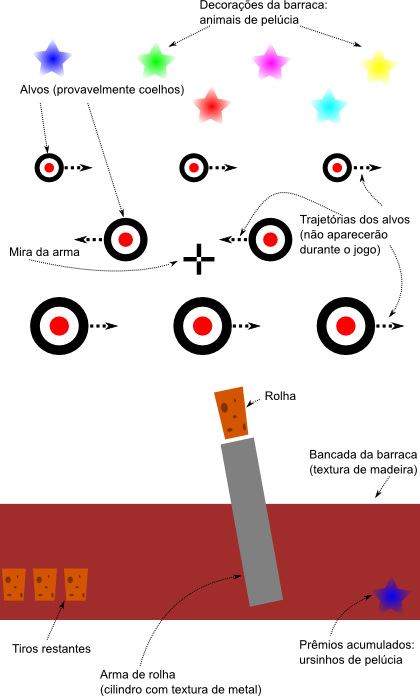
\includegraphics{barraca.png}
 \caption{Desenho conceitual da cena pela vis\~ao da c\^amera}
 \label{fig:barraca}
\end{figure}


\begin{figure}[htbp]
 \centering
  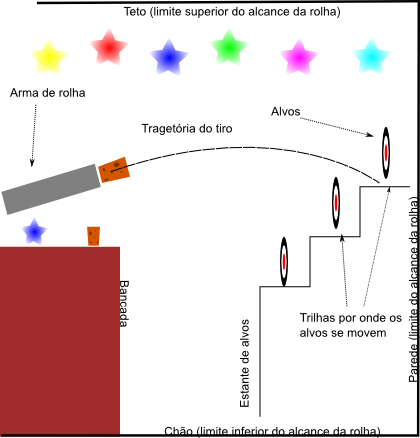
\includegraphics{lateral.png}
 \caption{Desenho conceitual da cena atrav\'es de um \^angulo lateral}
 \label{fig:lateral}
\end{figure}


\begin{figure}[htbp]
 \centering
  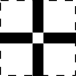
\includegraphics{mira.png}
 \caption{Exemplo de uma mira de tiro. A \'area tracejada indica a \'area por onde a rolha \'e lan\c cada com mais precis\~ao}
 \label{fig:mira}
\end{figure}


\begin{figure}[htbp]
 \centering
  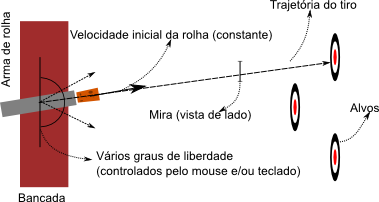
\includegraphics{tiro_cima.png}
 \caption{Rascunho do conceito da trajet\'oria da rolha - vis\~ao de cima}
 \label{fig:tiro_cima}
\end{figure}


\begin{figure}[htbp]
 \centering
  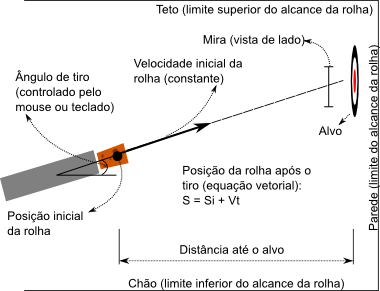
\includegraphics{movimento_linear.png}
 \caption{Rascunho do conceito da trajet\'oria linear da rolha - vis\~ao lateral}
 \label{fig:movimento_linear}
\end{figure}


\begin{figure}[htbp]
 \centering
  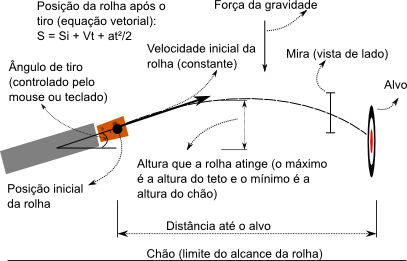
\includegraphics{movimento_parabolico.png}
 \caption{Rascunho do conceito da trajet\'oria parab\'olica da rolha - vis\~ao lateral}
 \label{fig:movimento_parabolico}
\end{figure}

\end{document}
